%% LyX 2.2.3 created this file.  For more info, see http://www.lyx.org/.
%% Do not edit unless you really know what you are doing.
\documentclass[english,12pt]{article}
\usepackage[T1]{fontenc}
\usepackage[latin9]{inputenc}
\usepackage{mathtools}
\usepackage{url}
\usepackage{amsmath}
\usepackage{amsthm}
\usepackage{amssymb}
\usepackage{graphicx}

\makeatletter
%%%%%%%%%%%%%%%%%%%%%%%%%%%%%% Textclass specific LaTeX commands.
\theoremstyle{plain}
\newtheorem{thm}{\protect\theoremname}[section]
\theoremstyle{definition}
\newtheorem{defn}[thm]{\protect\definitionname}
\theoremstyle{plain}
\newtheorem{prop}[thm]{\protect\propositionname}
\ifx\proof\undefined
\newenvironment{proof}[1][\protect\proofname]{\par
\normalfont\topsep6\p@\@plus6\p@\relax
\trivlist
\itemindent\parindent
\item[\hskip\labelsep\scshape #1]\ignorespaces
}{%
\endtrivlist\@endpefalse
}
\providecommand{\proofname}{Proof}
\fi
\theoremstyle{definition}
\newtheorem{example}[thm]{\protect\examplename}
\theoremstyle{plain}
\newtheorem{cor}[thm]{\protect\corollaryname}
\theoremstyle{plain}
\newtheorem{lem}[thm]{\protect\lemmaname}

%%%%%%%%%%%%%%%%%%%%%%%%%%%%%% User specified LaTeX commands.
\usepackage[margin=1in]{geometry}
\usepackage{tikz}
\usetikzlibrary{arrows,decorations.pathreplacing,shapes}

\makeatother

\usepackage{babel}
\providecommand{\corollaryname}{Corollary}
\providecommand{\definitionname}{Definition}
\providecommand{\examplename}{Example}
\providecommand{\lemmaname}{Lemma}
\providecommand{\propositionname}{Proposition}
\providecommand{\theoremname}{Theorem}

\begin{document}

\title{Math 525: Lecture 22}

\date{April 05, 2018}

\maketitle
In the last lecture, we showed that the running cost $v$ of a Markov
decision process satisfies a so-called \emph{Bellman} \emph{equation}:
\begin{equation}
\sup_{\pi_{0}\in\Pi_{0}}\left\{ \left(I-B(\pi_{0})\right)v-c(\pi_{0})\right\} =0\label{eq:original_bellman}
\end{equation}
where
\[
B(\pi_{0})=\begin{pmatrix}b_{1}(\pi_{0}(1))^{\intercal}\\
b_{2}(\pi_{0}(2))^{\intercal}\\
\vdots\\
b_{m}(\pi_{0}(m))^{\intercal}
\end{pmatrix}\text{with }b_{i}(\cdot)\geq0\text{ and }b_{i}(\cdot)^{\intercal}e\leq1\qquad\text{and}\qquad c(\pi_{0})=\begin{pmatrix}c(\pi_{0}(1),1)\\
c(\pi_{0}(2),1)\\
\vdots\\
c(\pi_{0}(m),m)
\end{pmatrix}.
\]
In the case of a fixed discount factor $0\leq d<1$, we saw that $B$
simplified to
\[
B(\pi_{0})=d\underbrace{\begin{pmatrix}p_{1}(\pi_{0}(1))^{\intercal}\\
p_{2}(\pi_{0}(2))^{\intercal}\\
\vdots\\
p_{m}(\pi_{0}(m))^{\intercal}
\end{pmatrix}}_{P(\pi_{0})}\text{ with }p_{i}(\cdot)\geq0\text{ and }p_{i}(\cdot)^{\intercal}e=1.
\]

In this lecture, we will establish uniqueness of a solution $v$ to
(\ref{eq:original_bellman}) and discuss how to compute it. Throughout,
we assume
\[
\Pi_{0}\text{ is a finite set}
\]
(i.e., there are only finitely many actions the controller can take
at each state). While this assumption can be relaxed, we do not do
so here. In this case, \ref{eq:original_bellman} becomes
\begin{equation}
\max_{\pi_{0}\in\Pi_{0}}\left\{ A(\pi_{0})v-c(\pi_{0})\right\} =0\qquad\text{where}\qquad A(\pi_{0})=I-B(\pi_{0}).\label{eq:bellman}
\end{equation}

\pagebreak{}

\section{Matrix classes}

First, we will need to recall some more linear algebra.

\subsection{Monotone matrices}
\begin{defn}
A \emph{monotone matrix} is a real square matrix $A$ such that $Ax\geq0$
implies $x\geq0$ for all real vectors $x$.
\end{defn}
\begin{prop}
Monotone matrices are nonsingular.
\end{prop}
\begin{proof}
Let $A$ be a monotone matrix and assume there exists $x$ with $Ax=0$.
Then, by monotonicity, $x\geq0$ and $-x\geq0$, and hence $x=0$.
\end{proof}
%
\begin{prop}
A real square matrix $A$ is monotone if and only if $A^{-1}$ exists
and is nonnegative.
\end{prop}
\begin{proof}
Suppose $A$ is monotone. Denote by $x$ the $i$-th column of $A^{-1}$.
Then, $Ax$ is the $i$-th standard basis vector, and hence $x\geq0$
by monotonicity. For the reverse direction, suppose $A$ admits a
nonnegative inverse. Then, if $Ax\geq0$, $x=A^{-1}Ax\geq A^{-1}0=0$,
and hence $A$ is monotone.
\end{proof}

\subsection{M-matrices}
\begin{defn}
An \emph{M-matrix} is any square matrix $A$ which can be written
in the form
\begin{equation}
A=sI-B\label{eq:m_matrix}
\end{equation}
where $s\geq\rho(B)$ and $B$ is nonnegative.
\end{defn}
\begin{prop}
\label{prop:m_matrix}The M-matrix (\ref{eq:m_matrix}) is nonsingular
if and only if $s>\rho(B)$.
\end{prop}
\begin{proof}
Note that $A$ is nonsingular if and only if $s$ is an eigenvalue
of $B$ since
\[
Ax=sx-Bx=0\iff Bx=sx.
\]
Therefore, if $s>\rho(B)$, then $A$ is nonsingular. Conversely,
if $s=\rho(B)$, by the Perron-Frobenius theorem, $s$ is an eigenvalue
of $B$.
\end{proof}
\begin{prop}
Nonsingular M-matrices are monotone.
\end{prop}
\begin{proof}
Divide (\ref{eq:m_matrix}) by $s$ so that
\[
s^{-1}A=I-s^{-1}B.
\]
Noting that $\rho(s^{-1}B)<1$, the inverse of the right hand side
of the above is the Neumann series
\[
\left(I-s^{-1}B\right)^{-1}=\sum_{k\geq0}\left(s^{-1}B\right)^{k}.
\]
In particular, this Neumann series consists only of powers of nonnegative
matrices, and therefore converges to a nonnegative matrix. In other
words, $sA^{-1}$ is nonnegative, and hence so too is $A^{-1}$.
\end{proof}

\subsection{Weakly chained diagonally dominant matrices}
\begin{defn}
Let $A=(A_{ij})\in\mathbb{C}^{m\times n}$ be a matrix. We say its
$i$-th row is \emph{strictly diagonally dominant} (s.d.d.) if
\begin{equation}
\left|A_{ii}\right|>\sum_{i\neq j}\left|A_{ij}\right|.\label{eq:sdd}
\end{equation}
We say the matrix is s.d.d. if all of its rows are s.d.d. Weakly diagonally
dominant (w.d.d.) is defined with weak inequality ($\geq$) instead.
\end{defn}
\begin{example}
The matrix
\begin{equation}
\begin{pmatrix}\phantom{-}1\\
-1 & \phantom{-}1\\
 & -1 & \phantom{-}1\\
 &  & -1 & \phantom{-}1
\end{pmatrix}\label{eq:matrix}
\end{equation}
is not strictly diagonally dominant, but it is weakly diagonally dominant.
\end{example}
\begin{defn}
\label{def:wcdd}Let $A=(A_{ij})\in\mathbb{C}^{m\times m}$ be a matrix.
Let \[ J = \{ i \colon i \text{ satisfies } \eqref{eq:sdd} \} \]
denote the set of all s.d.d. rows of $A$. We say $A$ is \emph{weakly
chained diagonally dominant} (w.c.d.d.) if
\begin{enumerate}
\item $A$ is w.d.d.
\item \label{enu:wcdd}For each row $i\notin J$, there is a walk $i\rightarrow j$
with $j\in J$.
\end{enumerate}
\end{defn}
\begin{example}
The matrix (\ref{eq:matrix}) is w.c.d.d. (see Figure \ref{fig:graph}).
\end{example}
\begin{figure}
\begin{centering}
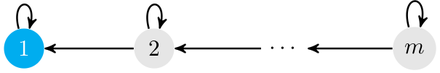
\includegraphics[width=3in]{wcdd}
\par\end{centering}
\caption{Graph of (\ref{eq:matrix})\label{fig:graph}}
\end{figure}

The following first appeared in Shivakumar, P. N., and Kim Ho Chew.
``A sufficient condition for nonvanishing of determinants.'' \emph{Proceedings
of the American Mathematical Society} (1974).
\begin{prop}
\label{prop:wcdd}w.c.d.d. matrices are nonsingular.
\end{prop}
\begin{proof}
Let $A$ be w.c.d.d. If $A$ is singular, we can find a nonzero vector
$x$ such that $Ax=0$. Without loss of generality, let $i_{1}$ be
such that $|x_{i_{1}}|=1\geq|x_{j}|$ for all $j$. Since $A$ is
w.c.d.d., we may pick a walk $i_{1}\dashrightarrow i_{2}\dashrightarrow\cdots\dashrightarrow i_{k}$
ending at an s.d.d. row $i_{k}\in J$.

Taking moduli on both sides of
\[
-a_{i_{1}i_{1}}x_{i_{1}}=\sum_{j\neq i_{1}}a_{i_{1}j}x_{j}
\]
yields
\[
\left|a_{i_{1}i_{1}}\right|=\left|a_{i_{1}i_{1}}x_{i_{1}}\right|=\left|\sum_{j\neq i_{1}}a_{i_{1}j}x_{j}\right|\leq\sum_{j\neq i_{1}}\left|a_{i_{1}j}\right|\left|x_{j}\right|\leq\sum_{j\neq i_{1}}\left|a_{i_{1}j}\right|.
\]
Since $A$ is w.d.d., the above must hold with equality. Therefore,
$|x_{j}|=1$ whenever $a_{i_{1}j}$ is nonzero. In particular, $|x_{i_{2}}|=1$,
and we can repeat the same argument as above to get that row $i_{2}$
is not s.d.d., row $i_{3}$ is not s.d.d., etc. until we conclude
that row $i_{k}$ is not s.d.d., a contradiction.
\end{proof}
\begin{figure}
\begin{centering}
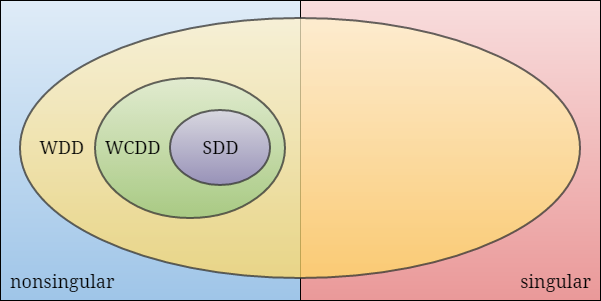
\includegraphics[width=4in]{wcdd_venn}
\par\end{centering}
\caption{Containment of matrix classes}
\end{figure}
\begin{thm}
\label{thm:wcdd}Let $A$ be a square w.d.d. matrix with nonnegative
diagonals ($A_{ii}\geq0$) and nonpositive off-diagonals (i.e., $A_{ij}\leq0$
for $i\neq j$). Then, the following are equivalent:
\begin{enumerate}
\item $A$ is a nonsingular M-matrix.
\item $A$ is a nonsingular matrix with positive diagonals.
\item $A$ is w.c.d.d.
\end{enumerate}
\end{thm}
Throughout the proof we use the fact that $A$ can be written in the
form $A=sI-B$ by taking $s=\max_{i}A_{ii}$, $B_{ii}=s-A_{ii}$,
and $B_{ij}=-A_{ij}$ for $j\neq i$. Since $A$ is w.d.d., this implies
\[
s-B_{ii}=A_{ii}\geq\sum_{j\neq i}\left|A_{ij}\right|=\sum_{j\neq i}B_{ij}
\]
and hence
\[
\rho(B)\leq\left\Vert B\right\Vert _{\infty}=\max_{i}\left\{ B_{ii}+\sum_{j\neq i}B_{ij}\right\} \leq\max_{i}\left\{ B_{ii}+s-B_{ii}\right\} =s.
\]
In other words, $A$ is a (possibly singular) M-matrix.
\begin{proof}[Proof of (1) $\implies$ (2)]
 It is sufficient to prove that if $A$ is nonsingular, then $A$
has positive diagonals. We prove the contrapositive. Suppose $A_{ii}=0$
for some $i$. Then, $|A_{ij}|=B_{ij}=0$ for all $j$. That is, the
$i$-th row of $A$ is zero, and hence $A$ is singular.
\end{proof}
%
\begin{proof}[Proof of (2) $\implies$ (3)]
 This proof is nontrivial, and hence I refer you to (self-plug) Azimzadeh,
P. ``A fast and stable test to check if a weakly diagonally dominant
matrix is a nonsingular M-matrix.'' \emph{Mathematics of Computation}
(2018).
\end{proof}
%
\begin{proof}[Proof of (3) $\implies$ (1)]
 If $A$ is w.c.d.d., it is nonsingular (Proposition \ref{prop:wcdd}).
\end{proof}
\begin{cor}
A square s.d.d. matrix with nonnegative diagonals and nonpositive
off-diagonals is a nonsingular M-matrix.
\end{cor}
\begin{proof}
An s.d.d. matrix is a w.c.d.d. matrix.
\end{proof}

\section{Bellman equation}

We start with a trivial observation.
\begin{lem}
$A(\pi_{0})$ is a square w.d.d. matrix with nonnegative diagonals
and nonpositive off-diagonals.
\end{lem}
\begin{proof}
This is a result of the following observations:
\begin{itemize}
\item $(B(\pi_{0}))_{ii}\leq1$ so that $(A(\pi_{0}))_{ii}=1-(B(\pi_{0}))_{ii}\geq0$,
\item $(B(\pi_{0}))_{ij}\geq0$ so that $(A(\pi_{0}))_{ij}=-(B(\pi_{0}))_{ij}\leq0$
whenever $i\neq j$, and
\item $\sum_{j}(B(\pi_{0}))_{ij}\leq1$ so that $\sum_{j}(A(\pi_{0}))_{ij}=1-\sum_{j}(B(\pi_{0}))_{ij}\geq0$.\qedhere
\end{itemize}
\end{proof}
The above implies that we can quickly check to see if $A(\pi_{0})$
is a nonsingular M-matrix (and hence monotone) by verifying if it
is w.c.d.d. In the constant discount factor case, $A(\pi_{0})$ is
trivially w.c.d.d.:
\begin{example}
Suppose $A(\pi_{0})=I-dP(\pi_{0})$ for some $0\leq d<1$. Then,
\[
\sum_{j}(A(\pi_{0}))_{ij}=1-d\sum_{j}(P(\pi_{0}))_{ij}=1-d>0.
\]
In other words, $A(\pi_{0})$ is s.d.d. since $(A(\pi_{0}))_{ii}>\sum_{j\neq i}|(A(\pi_{0}))_{ij}|$.
\end{example}

\subsection{Uniqueness}
\begin{thm}
Suppose $A(\pi_{0})$ is w.c.d.d. for each $\pi_{0}$. Then, solutions
of (\ref{eq:bellman}) are unique.
\end{thm}
\begin{proof}
Let $v$ and $v^{\prime}$ satisfy equation (\ref{eq:bellman}). Pick
$\pi_{0}^{v}$ such that
\[
0=\max_{\pi_{0}\in\Pi_{0}}\left\{ A(\pi_{0})v-c(\pi_{0})\right\} =A(\pi_{0}^{v})v-c(\pi_{0}^{v}).
\]
Then,
\[
0=\max_{\pi_{0}\in\Pi_{0}}\left\{ A(\pi_{0})w-c(\pi_{0})\right\} \geq A(\pi_{0}^{v})w-c(\pi_{0}^{v}).
\]
Putting these two together,
\[
A(\pi_{0}^{v})\left(v-w\right)\geq0.
\]
Since $A(\pi_{0}^{v})$ is monotone, its inverse exists and is nonnegative.
Therefore, we can multiply both sides of the above inequality by $(A(\pi_{0}^{v}))^{-1}$
to get $v-w\geq0$. Switching the roles of $v$ and $w$ in this argument,
we get $w-v\geq0$.
\end{proof}

\subsection{Policy iteration}

One way to compute the solution $v$ is by the so-called \emph{policy
iteration algorithm}:
\begin{enumerate}
\item Pick an ``initial guess'' $\pi_{0}^{(0)}\in\Pi_{0}$. Set $v^{(0)}=(-\infty,\ldots,-\infty)$
and $k\gets1$.
\item Solve the linear system $A(\pi_{0}^{(k-1)})v^{(k)}=b(\pi_{0}^{(k-1)})$
for $v^{(k)}\in\mathbb{R}^{m}$.
\item Pick $\pi_{0}^{(k)}\in\Pi_{0}$ such that $A(\pi_{0}^{(k)})v^{(k)}-b(\pi_{0}^{(k)})=\max_{\pi_{0}\in\Pi_{0}}\{A(\pi_{0})v^{(k)}-b(\pi_{0})\}$.
\item If $v^{(k)}=v^{(k-1)}$, \textbf{stop}. Otherwise, set $k\gets k+1$
and \textbf{go to} step 2.
\end{enumerate}
\begin{thm}
Suppose $A(\pi_{0})$ is w.c.d.d. for each $\pi_{0}$. Then, the above
policy iteration algorithm converges to the solution $v$ of (\ref{eq:bellman})
in at most $|\Pi_{0}|$ iterations (i.e., $v=v^{(|\Pi_{0}|)}=v^{(|\Pi_{0}|+1)}=\cdots$).
\end{thm}
\begin{proof}
A nice reference for this fact is Bokanowski, Olivier, Stefania Maroso,
and Hasnaa Zidani. ``Some convergence results for Howard's algorithm.''
\emph{SIAM Journal on Numerical Analysis} 47.4 (2009): 3001-3026.
\end{proof}

\subsection{Example}

\begin{figure}
\begin{centering}
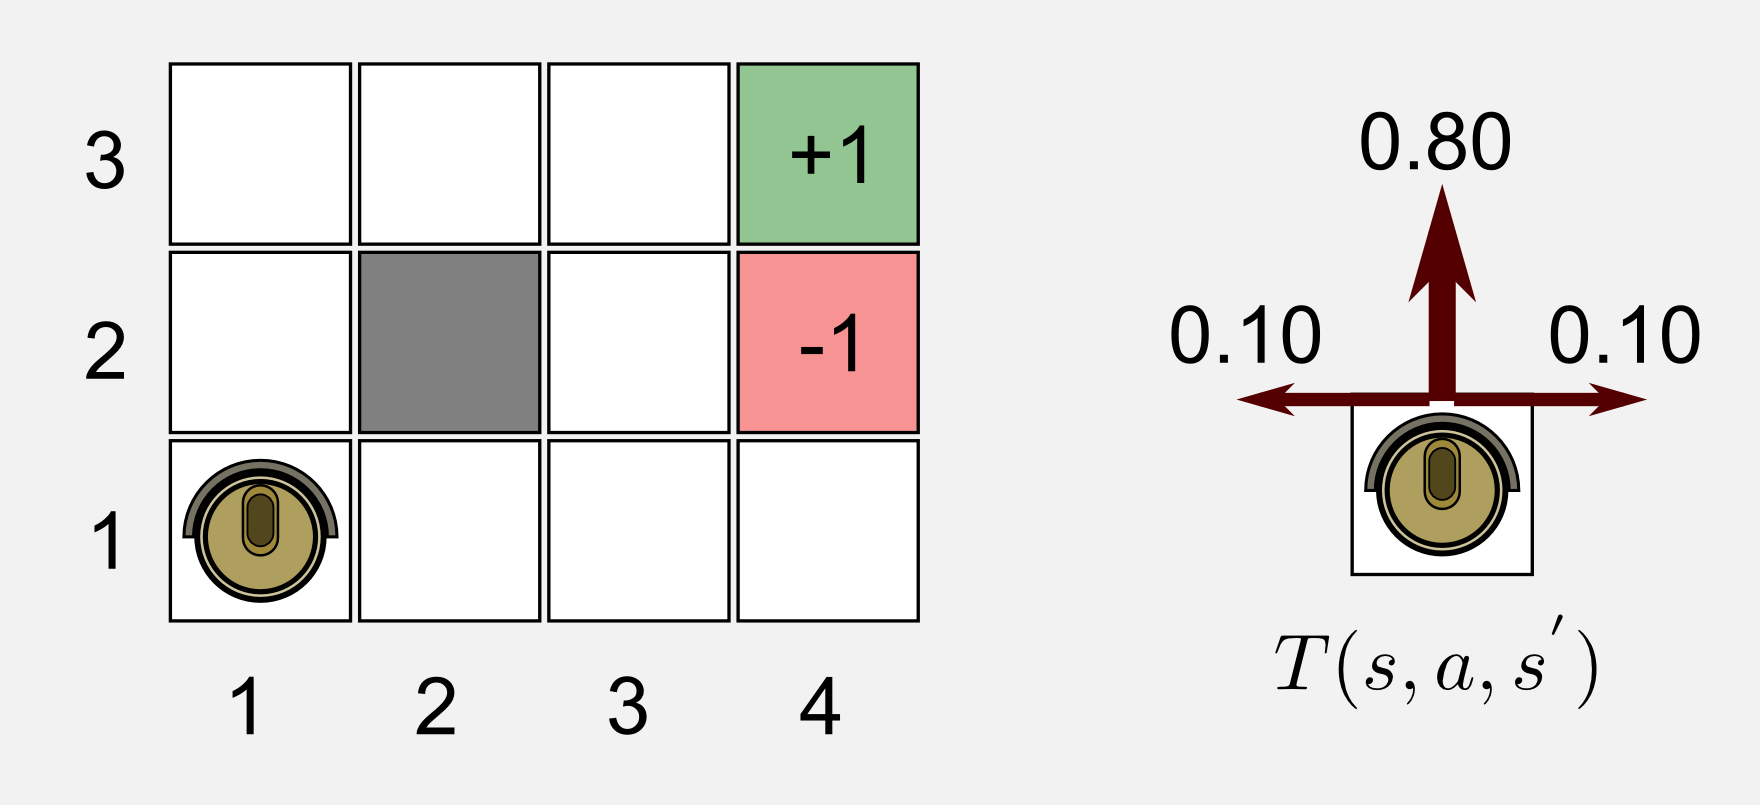
\includegraphics[width=4in]{robot}
\par\end{centering}
\caption{Robot navigation}
\end{figure}
\begin{itemize}
\item This example is by Massimiliano Patacchiola (\url{https://mpatacchiola.github.io/}).
\item A robot, started in position $(1,1)$, has to find the best way to
reach the charging station (Reward +1) and to avoid falling down the
flight of stairs (Reward -1).
\item This is a Markov chain with state space $S=\{(1,1),(1,2),\ldots,(4,3),\emptyset\}$
($\emptyset$ is an extra state which both $(4,3)$ and $(4,2)$ transition
to deterministically to signify the end of the game).
\item At each state $i$, the robot gets to choose which direction to face:
$\mathcal{A}_{i}=\{N,S,W,E\}$. Then, the robot tries to move forward.
However, being faulty, 10\% of the time it moves to its left and 10\%
of the time it moves to its right. This determines the transition
matrix $P(\pi_{0})$.
\item The reward function is $r(i)=I_{\{(4,3)\}}(i)-I_{\{(4,2)\}}(i)$.
\item We take a discount factor of $d=0.999<1$ so that $A(\pi_{0})=I-dP(\pi_{0})$.
\item The Markov decision process is
\[
\underbrace{\max_{\pi\in\Pi}\mathbb{E}\left[\sum_{n\geq0}0.999^{n}r(X_{n}^{\pi})\right]}_{\text{maximize rewards }r}=-\underbrace{\min_{\pi\in\Pi}\mathbb{E}\left[\sum_{n\geq0}0.999^{n}(-r(X_{n}^{\pi}))\right]}_{\text{minimize costs }c=-r}
\]
\end{itemize}
\begin{figure}
\begin{centering}
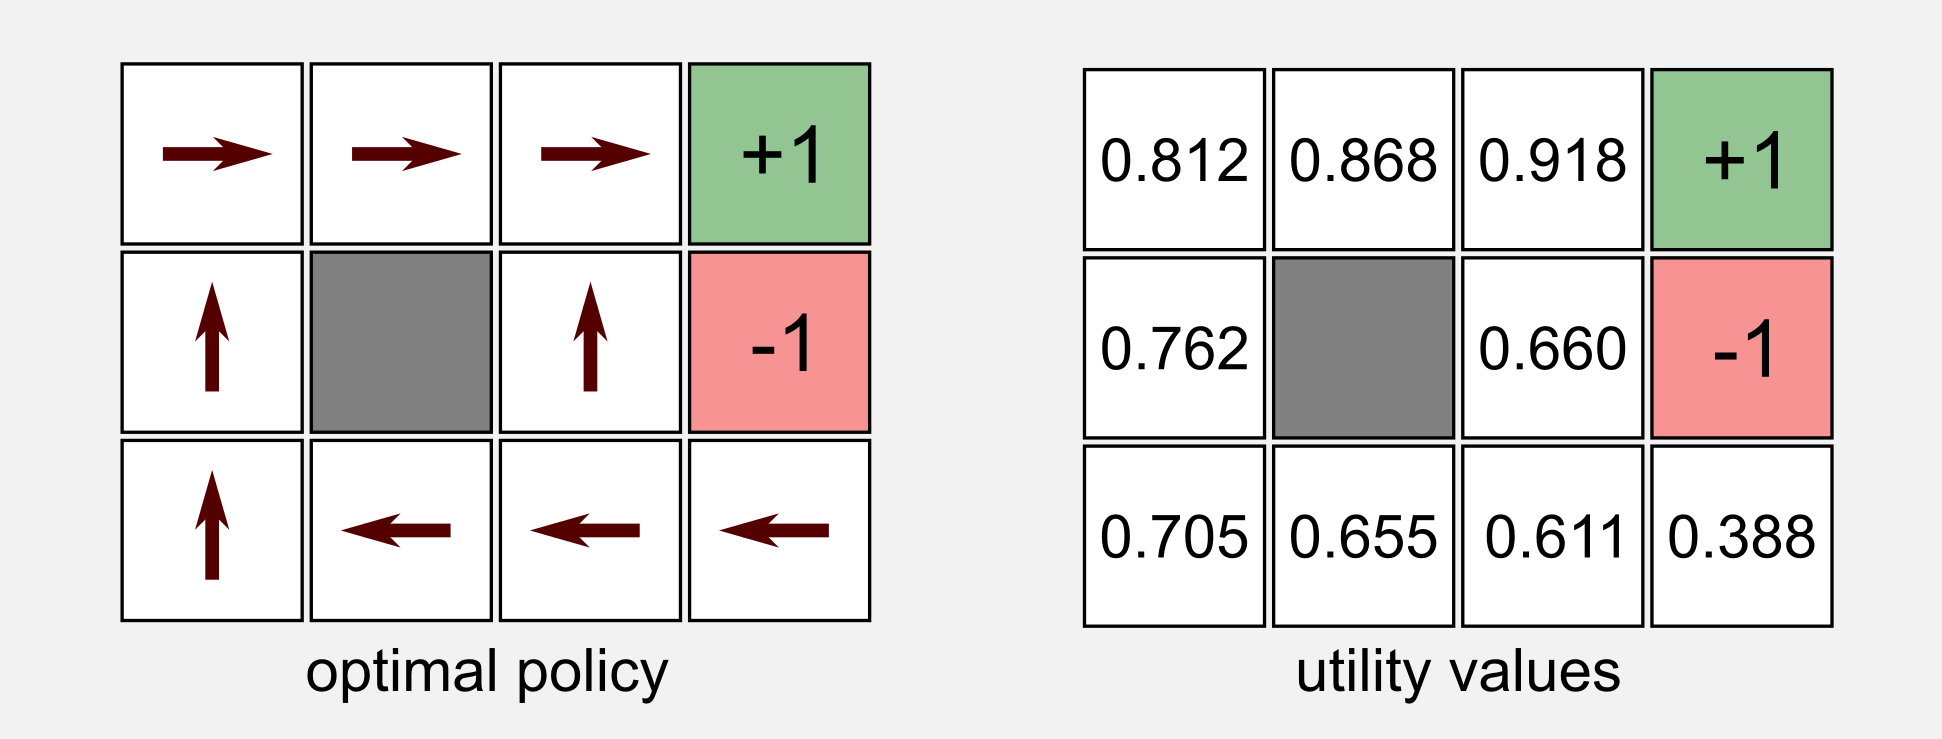
\includegraphics[width=4in]{robot_optimal}
\par\end{centering}
\caption{Result of running policy iteration}
\end{figure}

\end{document}
